

{\centering
\begin{figure}
  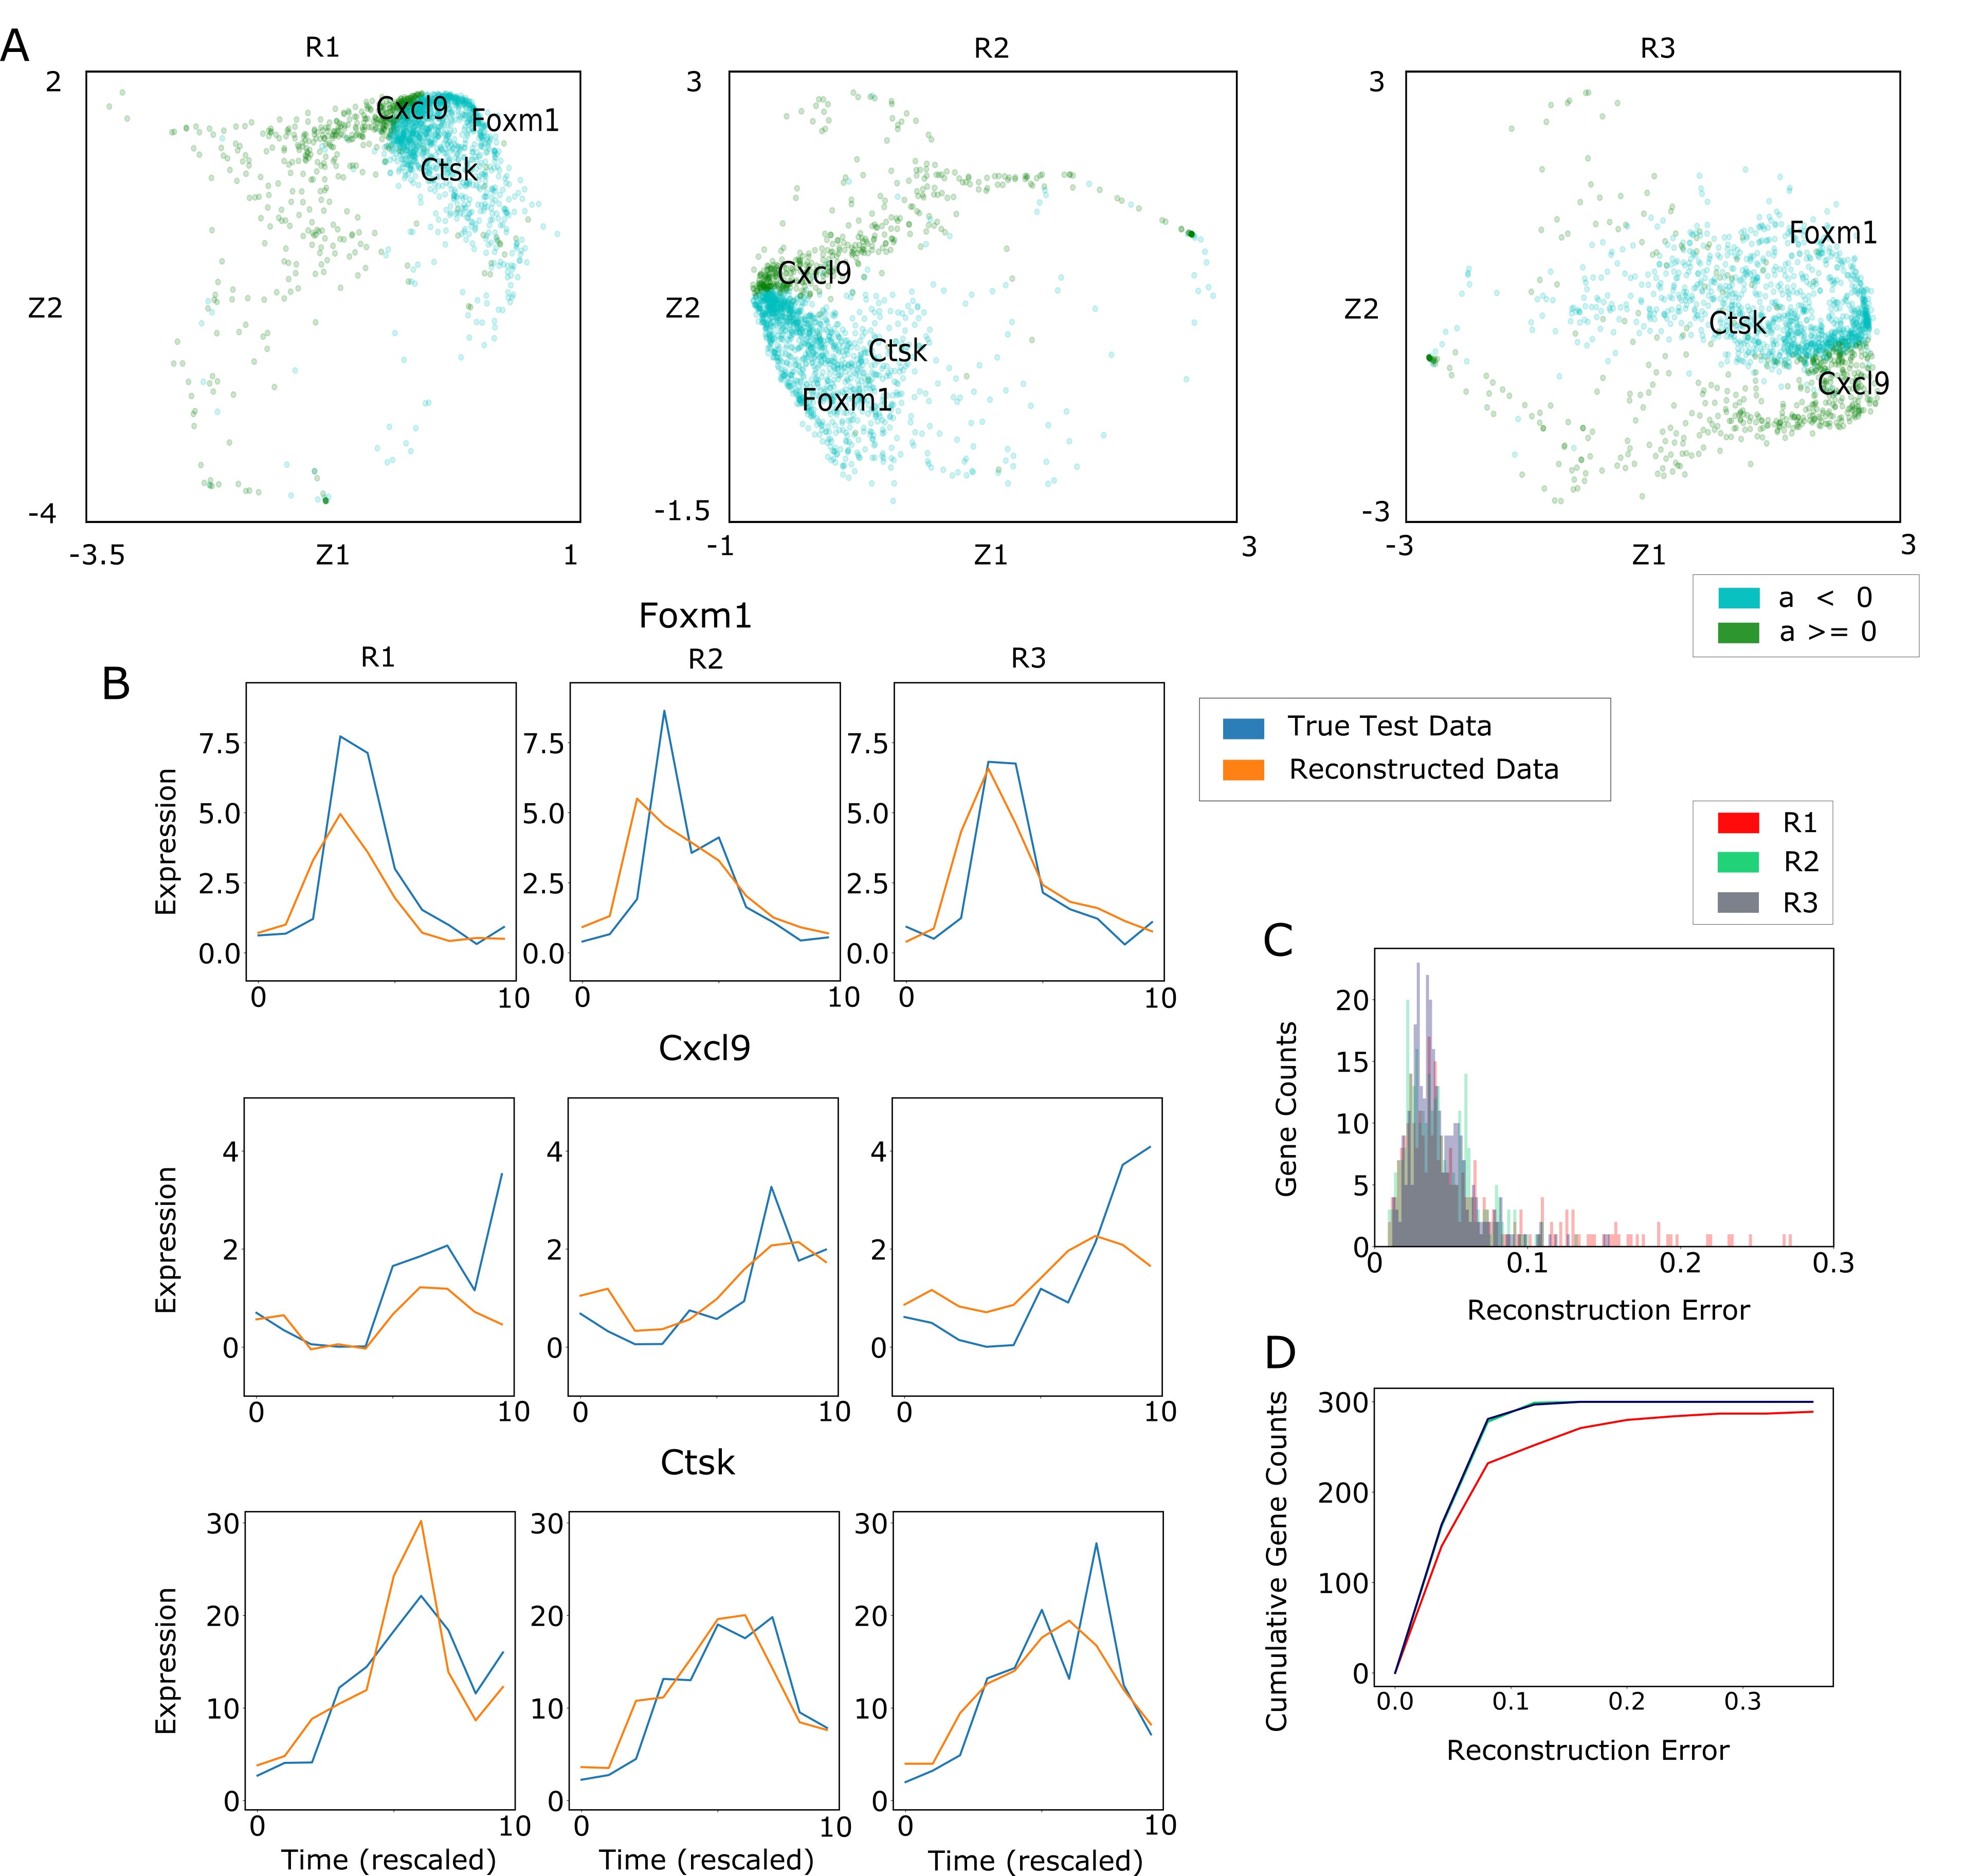
\includegraphics[width = \linewidth]{figures/quad_jci.png}
 % archetecture.png: 1149x508 px, 72dpi, 40.53x17.92 cm, bb=0 0 1149 508
    \caption[Accurate reconstruction of kidney injury response gene dynamics with RVAgene.]{{\bf Accurate reconstruction of kidney injury response gene dynamics with RVAgene. (A)} Latent space representations of RVAgene models trained separately on three independent replicates (R1-R3); classified by quadratic fit coefficient $a$. ({\bf B}) Model generation of gene dynamics for genes not used in training: {\em Foxm1, Cxcl9} and {\em Ctsk}. ({\bf C}) Histograms of reconstruction errors for RVAgene models trained on R1-R3 (truncated). ({\bf D}) Cumulative distribution of reconstruction errors. }
  \label{fig:fig6a}
\end{figure}
}



\subsection{RVAgene can classify and predict gene expression dynamics in response to kidney injury}

We investigated gene expression dynamics in the murine kidney by applying RVAgene to a dataset that describes gene expression profiles before, during, and after a kidney injury \citep{liu2017molecular}. The dataset is temporally rich, with a total of ten bulk samples over twelve months. Since in this case no single-cell information is available, we cannot order samples by pseudotime to smooth the data. Moreover, the temporal gene expression profiles described in \citet{liu2017molecular} display more complex dynamics than for the previous dataset \citep{Klein2015}, and are not readily separable by linear patterns of up- and down-regulated genes (cf. \hyperref[fig:fig3]{Fig. 2C}). Thus, below, we must consider nonlinear models in order to characterize the temporal patterns observed.
\par 
The data consist of one initial timepoint ($t = 0$) before the injury event (an ischemia/reperfusion injury model) and nine subsequent time points ($t = 1$ to $10$) following the injury (48 hours, 72 hours, 7 days, 14 days, 28 days, 6 months and 12 months). We note that the timepoints are not uniformly spaced, which is not taken into account in RVAgene, which only models the broad temporal trend (see Discussion). From an initial list of 1927 differentially expressed genes measured over the time course in three biological replicates, we removed putative/predicted and non-protein coding genes, retaining a list of 1713 genes as input to the model.
\par 
We ran RVAgene separately for each of three biological replicates. Independent replicates \& independently trained models provide additional means with which to test the reproducibility of these methods. For each replicate, RVAgene was trained with a two-dimensional latent space and a hidden size of 10, on the full set of genes over 200 epochs: found to be sufficient for the convergence of $\cL$ (see Methods for further details). We fit linear regression models to the temporal gene profiles (\hyperref[supp]{Fig. S5}) and found that linear fits rarely described the gene temporal profiles well (most correlation coefficients had values close to zero), not did they identify separate clusters in the latent space. Normalizing the data to lie in $[0,1]$ improved our ability to discriminate clusters in the latent space (\hyperref[supp]{Fig. S5C}), but came at the expense of a significant loss of information, as the variance captured in the latent space was dramatically reduced. The absence of evidence for linear correlations could indicate expression dynamics that are uncorrelated with time, but could of course also indicate more complicated (nonlinear) gene expression dynamics, which are explored below. 
\par
To study nonlinear gene expression dynamics, we fit a 2nd degree polynomial, i.e. we fit the temporal trajectory of each gene $x$ to:  $x = at^2 + bt + c$, where $a,b,c$ are constants (\hyperref[supp]{Fig. S6}). We hypothesized that this function could adequately describe the transient dynamics observed by \citet{liu2017molecular} for most genes in response to the kidney injury. 
% Our hypothesis was that this model would be sufficient to capture simple patterns commonly observed during and following kidney injury, where the expression of a gene either increases or decreases transiently, before returning to near-baseline expression values.
Thus, we classified genes into one of two groups, $a < 0$: convex (up-down pattern), 1200 genes; and $a \geq 0$: concave (down-up pattern), 512 genes. In the latent space, the separation of these two groups is clearly visible for each replicate (\hyperref[fig:fig6a]{Fig. 4A}). Moreover, the classification is in agreement with \citet{liu2017molecular}, where the majority of differentially expressed genes are upregulated transiently. 
To explore the ability of RVAgene to reconstruct gene expression profiles not used in model development, we kept aside 300 randomly sampled genes for testing, and trained RVAgene models on the remaining genes for each of the three replicates. Independently for each model, we then generated dynamic profiles for the test genes. Three genes sampled randomly from the test set are plotted in \hyperref[fig:fig6a]{Fig. 4B}. Of particular note, for each of genes, the model-generated data captures the temporal patterns while displaying a higher degree of similarity across replicates than the experimental data itself. This illustrates that the model is neither under- nor overfitting, but capturing the underlying biological patterns while sufficiently accounting for the noise. 
%An interesting point to note is that for each of the shown example genes, the three separately trained RVAgene models for the three replicates come up with similar looking reconstructions although the actual data of the three replicates have different variations (while conforming with the general dynamics common to the three replicates).
Reconstruction errors are comparable across the three replicates, albeit with slightly higher overall errors in replicate 1 (\hyperref[fig:fig6a]{Fig. 4C-D}). Overall, the reconstruction errors are higher than for the previous section (averaging over many pseudotemporal time points allowed us to significantly reduced the noise). 



{\centering
\begin{figure}
  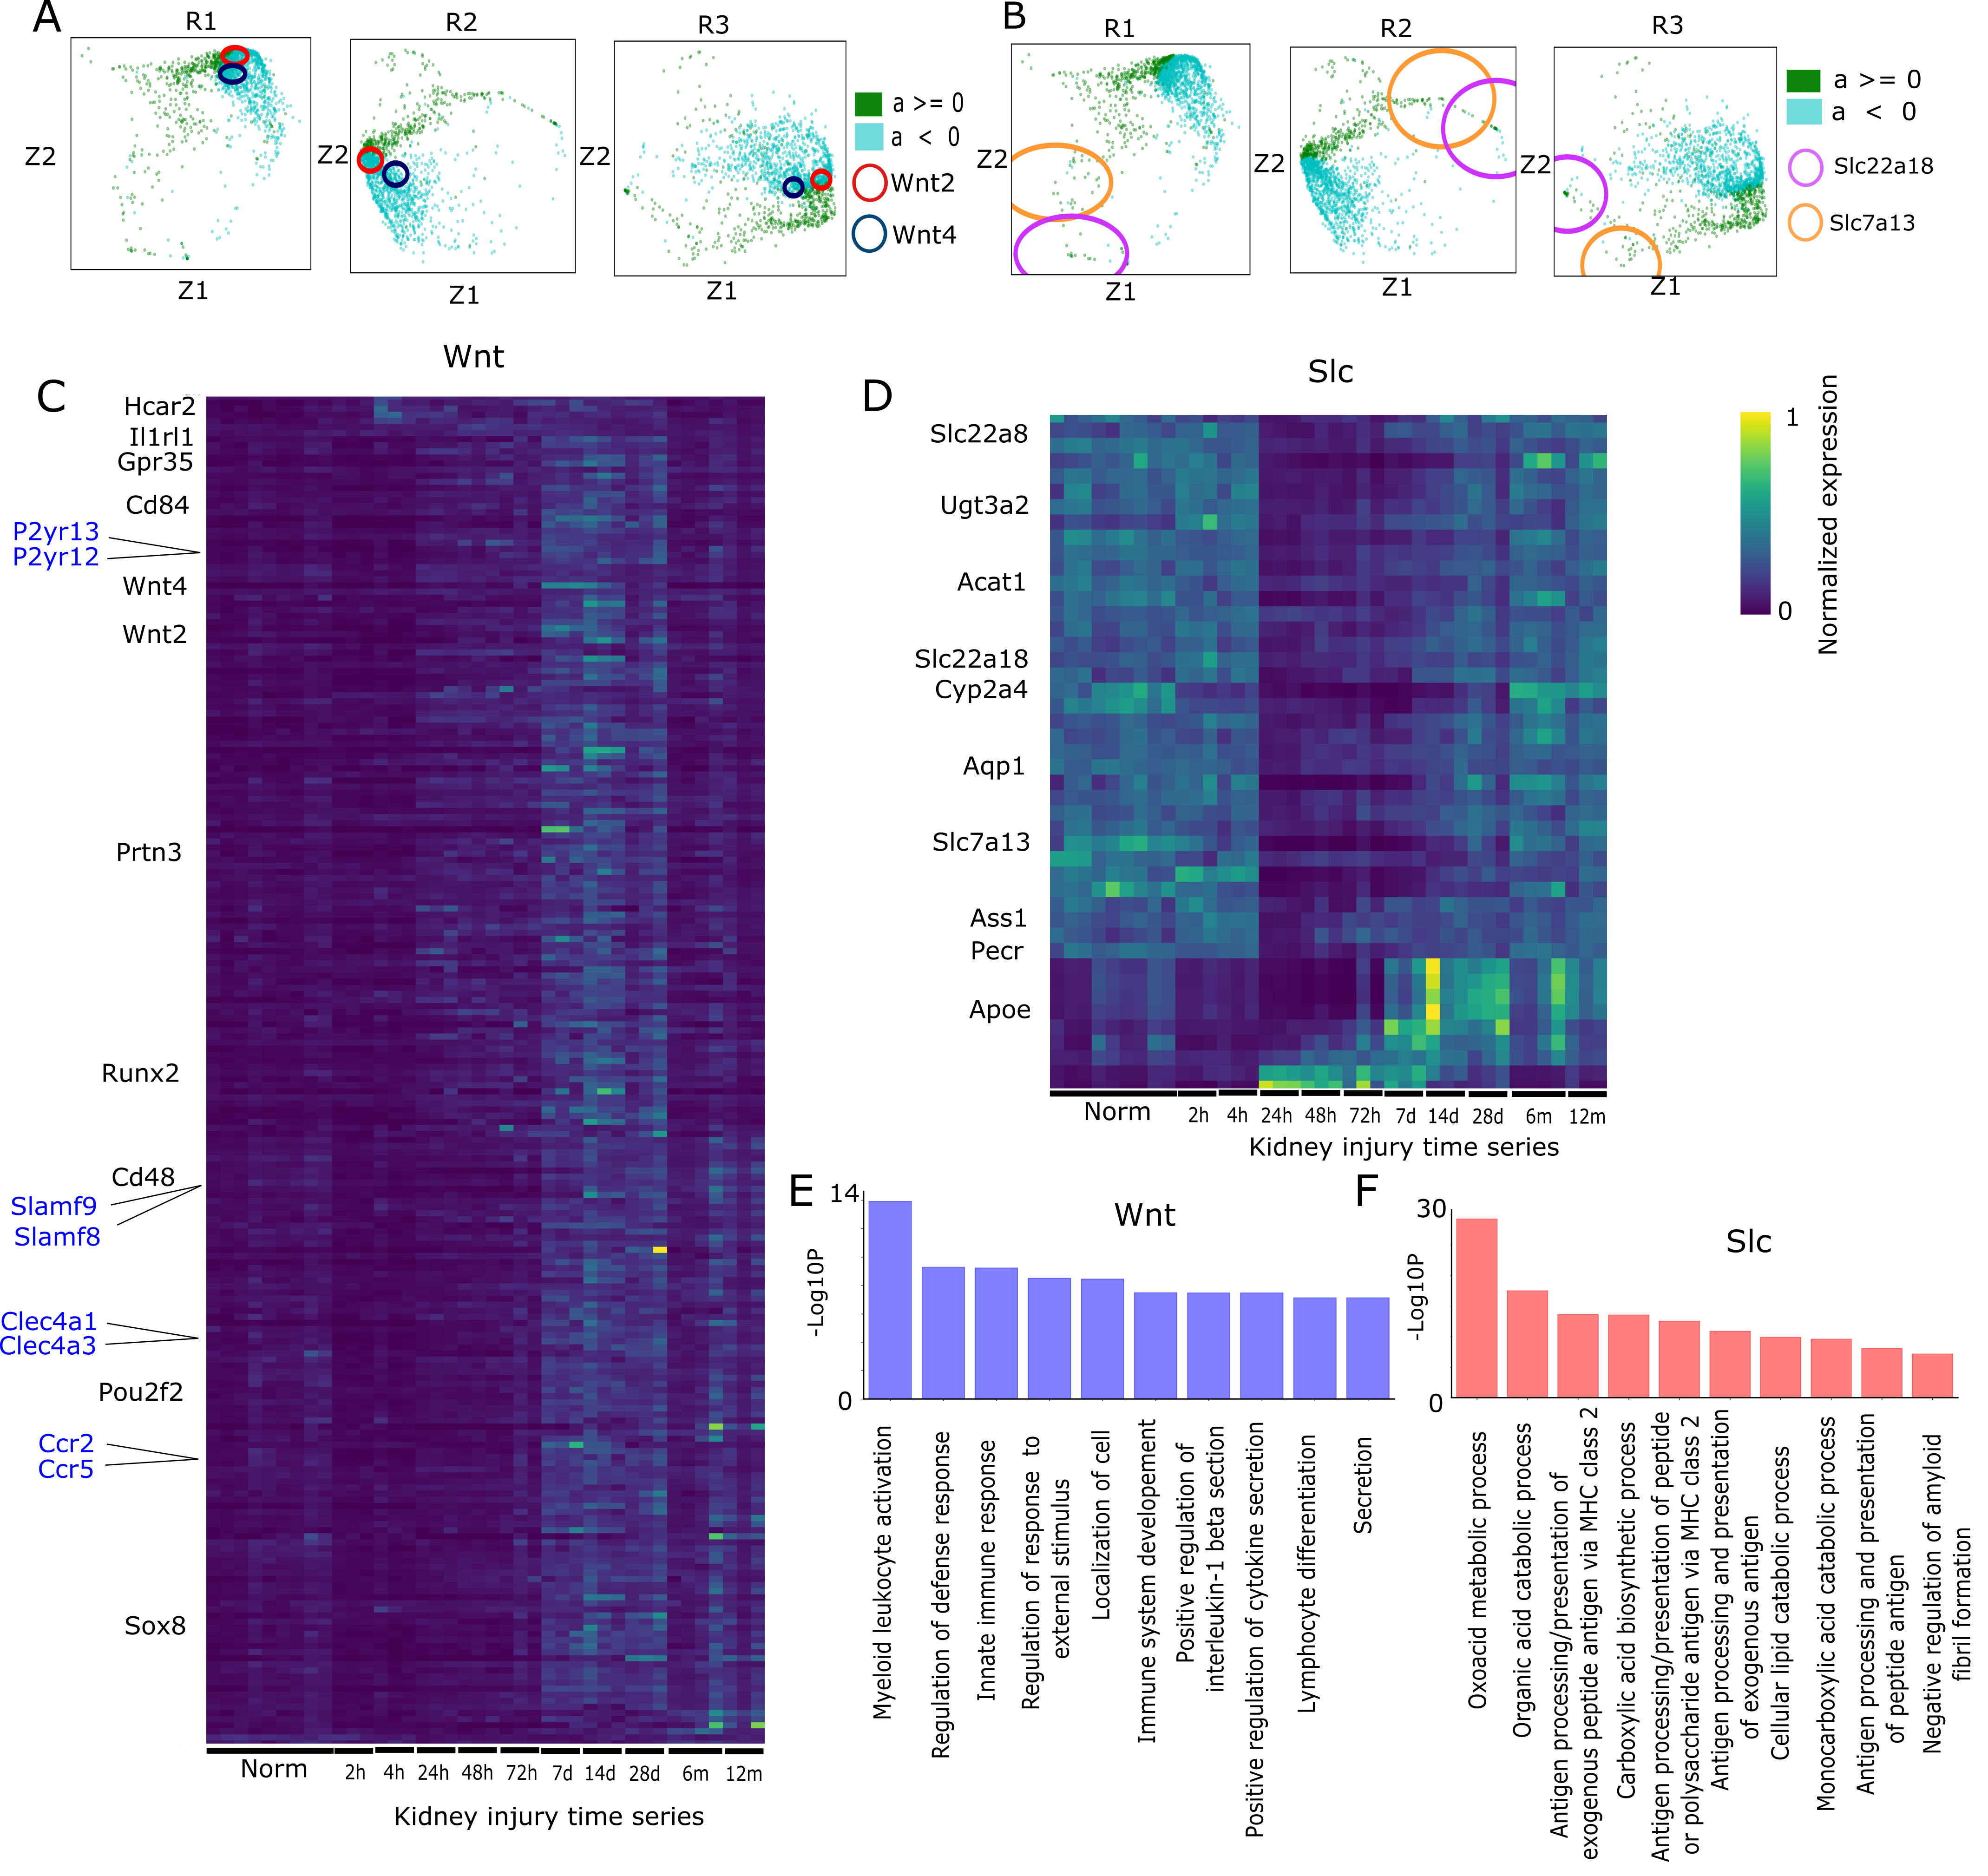
\includegraphics[width = \linewidth]{figures/fig9.png}
 % archetecture.png: 1149x508 px, 72dpi, 40.53x17.92 cm, bb=0 0 1149 508
    \caption[RVAgene latent space captures biological processes driving concordant gene expression changes.]{{\bf RVAgene latent space captures biological processes driving concordant gene expression changes. (A)} Z-plots for replicates R1-R3 with local neighborhoods of Wnt2 and Wnt4 marked (circles). ({\bf B}) As in A, for Slc family members Slc22a18 and Slc7a13. ({\bf C}) Heatmap of expression changes over time course of injury for the Wnt neighborhood genes in the intersection of R1-R3. Selected genes marked (black), as well as ortholog gene pairs (blue).  ({\bf D}) As in C, for Slc neighborhood genes. ({\bf E}) Histogram of -log10 p values of gene ontology terms for biological processes terms associated with the Wnt neighborhood (gene set in C). ({\bf F}) As in E, with the Slc neighborhood (gene set in D). }
  \label{fig:fig6b}
\end{figure}
}

{
  To investigate in more depth the features that are captured in the RVAgene latent space, we performed two sets of analyses: unbiased clustering, and targeted exploration. For the unbiased analysis, we performed k-means clustering on RVAgene latent space of replicate 1 (R1) with $k=9$ (Supplementary \hyperref[supp]{Fig. S7A}); we project the clusters labels learnt onto replicates R2 and R3. All cluster identities are well-preserved across replicates, with the exception of cluster 5, which seems to indicate outlier genes in R1. To study biological processes within these clusters, we performed GO term enrichment analysis on each. In Supplementary  \hyperref[supp]{Fig. S7B} we plot one significant GO term per cluster (omitting cluster 5), and see that specific regions of the latent spaces across replicates can be characterized in terms of biological processes, many of which relate to metabolic and immune system responses. These can be separated into two broad classes, which separate the left-hand side of R1 (metabolic processes downregulated during injury response) from the right-hand side (immune responses upregulated during injury response). 
}
\par 
To study the effects of gene-specific regions of the latent space in greater depth, we chose three distinct regions based on the co-location of genes of interest. These gene groups studied on the latent space are: 1) a {\em Wnt} group consisting of family members {\em Wnt2} \& {\em Wnt4}; 2) an {\em Slc} group consisting of family members {\em Slc7a13} \& {\em Slc22a18}; and 3) a {\em Sdc1} group, consisting of only {\em Sdc1}. For each group, we characterized neighboring genes by defining a circular neighborhood around each gene in the group, with radius $r$ (depending on the local density, the radius was varied, giving: $r^2 = 1$ for {\em Slc}, $r^2 = 0.3$ for {\em Sdc}, $r^2 = 0.05$ for {\em Wnt}. We then took all genes inside this radius for each replicate, and found the intersection of genes over the three replicates (\hyperref[fig:fig6b]{Fig. 5A-B}). We analyzed the intersection gene set for each group by studying their temporal profiles and their gene ontology (GO) term associations. Each group was characterized by a strikingly clear temporal profile. The {\em Sdc1} and {\em Wnt} groups both show transient upregulation, over different timescales: the {\em Sdc1} group is upregulated from 24 hours post-injury until 14-28 days post-injury (fast response) (Supplementary \hyperref[supp]{Fig. S8B}), whereas the {\em Wnt} group is upregulated at 7 days post-injury until 28 days post-injury (slow response) (\hyperref[fig:fig6b]{Fig. 5C}). In contrast, the {\em Slc} group is downregulated at 24 hours post-injury, and remains suppressed until 7-28 days post-injury (\hyperref[fig:fig6b]{Fig. 5D}).
\par 
Analysis of GO biological process terms enriched in each gene group further highlighted the power of the latent space for biological discovery. The fast response ({\em Sdc1}) group was characterized by upregulation of programs related to apoptosis, stress response, wound healing and chemotaxis, i.e. the first responders to the site of injury (\hyperref[supp]{Fig. S8C}). In addition all five {\em Lox} genes comprising the GO term ``peptidyl-lysine oxidization'' were found in this group. This is consistent with the oxidative stress resulting from the renal ischemia-reperfusion injury that was performed. However, distinct factors regulate the {\em Lox} family genes, as can be partly observed by their subtle differences in temporal profile (\hyperref[supp]{Fig. S8D}). Their co-location in the latent spaces of all three models thus highlights the potential use of RVAgene for discovery of complex temporal regulatory events from gene expression data.
\par
The slow response ({\em Wnt}) group was primarily characterized by immune response processes, including leukocyte activation, platelet aggregation, and various cytokine-mediated pathways including {\em IL-1} and {\em IL-33} (\hyperref[fig:fig6b]{Fig. 5E}). Notably, the Wnt group identies multiple gene orthologs (\hyperref[fig:fig6b]{Fig. 5C}) with very similar profiles: likely evidence of shared temporal regulation. This illustrates once again (as for the {\em Lox} genes above) the potency of RVAgene for the discovery of temporally co-regulated genes.
\par
Finally, the {\em Slc} group of genes shows a transiently down-regulated pattern between 24 hours and 7-28 days, although some gene in this group deviate from this pattern (\hyperref[fig:fig6b]{Fig. 5D}). 
GO term enrichment identifies the positive regulation of metabolic processes (\hyperref[fig:fig6b]{Fig. 5F}). The downregulation of metabolic programs during the response to kidney injury is agreement with the findings of \citet{liu2017molecular}. Notably, this metabolism-sensitive group contains many genes that also display sexually dimorphic expression, primarily in specific regions of the proximal tubule \citep{ransick19_singlecell}, thus independently identifying the well-established (though under-studied) interplay between sex differences and injury responses in the kidney \citep{neugarten00_effect}. 
\par 
In summary, unsupervised analysis of groups of genes co-located in the latent spaces of RVAgene finds: 1) high similarity between temporal gene profiles of genes nearby in latent space, and 2) clear biological signatures represented by these groups of nearby genes, in strong agreement with prior knowledge \citep{liu2017molecular}. Moreover, the latent spaces of RVAgene models can be used to predict programs of temporal co-regulation. 
\par


% In the latent space representation for all those genes and for the three replicates. We can see genes with positive and negative correlation between expression and time axis are not as distinctly separated as previous section, which is expected (Supplementary \hyperref[supp]{Fig. S2-B}). 
% This also hints that this dataset might not have clear cluster structures and an uninformed clustering effort on this dataset might produce forced spurious results. Now, one might think that the correlation measure is a measure of shape and somehow magnitude of expression of genes is playing part here (i.e. may be genes with similar dynamics but different scale of magnitudes are being viewed differently). Which means, normalising the expression magnitudes across timepoints to the same range (e.g. 0-1) might be helpful to increase the clarity of separation between the red and blue class. This indeed works as can be seen in supplementary \hyperref[supp]{Fig. S2-C}. However, it drastically reduces the variance in the latent space which can be inferred from the hugely shrunken scales of the axes from supplementary \hyperref[supp]{Fig. S2-B} to supplementary \hyperref[supp]{Fig. S2-C} for both dimensions of latent space i.e. a lot of important information is lost. This might not be a problem for the representation learning part, but, it means the decoder will be hugely underfit. So, we do not recommend normalising the data without any solid reason for the same. Another possibility is increasing the dimension of latent space. A 3D latent space could be better in this case but increasing it beyond 3 defeats the purpose of representation learning because each gene has only 10 timepoints anyway and latent space with more than 3 dimension will require dimensionality reduction for visualization.
 
%%% Local Variables:
%%% mode: latex
%%% TeX-master: t
%%% End:
